\documentclass[12pt,a4paper, twoside]{article}
\usepackage[utf8]{inputenc}
\usepackage{amsmath}
\usepackage{amsfonts}
\usepackage{amssymb}
\usepackage{graphicx}
\author{Marco Bertenghi}
\usepackage{amsthm}
\date{}
\usepackage{subfiles}
\usepackage[centering, a4paper]{geometry}
\usepackage{fancyhdr}
\pagestyle{fancy}

\fancyhead[RE]{\rightmark}
\fancyhead[RO]{}
\fancyhead[LO]{\leftmark}
\fancyhead[LE]{}

\newtheorem{lem}{Lemma}[section]
\newtheorem{thm}{Theorem}[section]
\newtheorem{prop}{Proposition}[section]
\newtheorem{cor}{Corollary}[section]
\newtheorem{defn}{Definition}[section]
\newtheorem{exmp}{Example}[section]
\theoremstyle{definition}
\newtheorem{rem}{Remark}[section]


\usepackage{color}  
\usepackage{hyperref}
\hypersetup{
    colorlinks=false, %set true if you want colored links
    linktoc=all,     %set to all if you want both sections and subsections linked
    linkcolor=blue,  %choose some color if you want links to stand out
}

\newenvironment{rcases}
  {\left.\begin{aligned}}
  {\end{aligned}\right\rbrace}

\graphicspath{{bmconst/}, {bmmarkov/},{bmdirichlet/}, {bmdonsker/}, {bmquadvar/}}



\begin{document}


\begin{titlepage}
	\centering
	
	{\scshape\LARGE University of Zurich \par}
	\vspace{2cm}
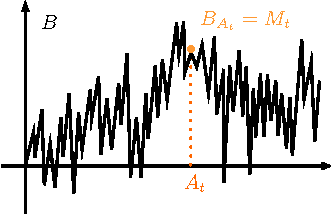
\includegraphics[width=.8\textwidth]{logo.pdf}\par\vspace{1cm}
	\vspace{1cm}
	{\huge\bfseries Brownian Motion\par}
	\vspace{2cm}
	{\Large\itshape Marco Bertenghi\par}
	\vfill
	Based on the lecture notes of \par
	Prof. Wendelin \textsc{Werner} (ETHZ)

	\vfill

% Bottom of the page
	{\large \today\par}
\end{titlepage}
\newpage


\tableofcontents

\newpage



\subfile{bmconst/bmconst.tex}
\newpage
\subfile{bmmarkov/bmmarkov.tex}
\newpage
\subfile{bmdirichlet/bmdirichlet.tex}
\newpage
\subfile{bmdonsker/donsker.tex}
\newpage
\subfile{bmcontmart/contmart.tex}
\newpage
\subfile{bmquadvar/bmquadvar.tex}
\newpage
\subfile{bmstochint/bmstochint.tex}
\newpage
\subfile{bmitoformula/bmitoformula.tex}
\newpage
\subfile{bmsde/bmsde.tex}
\newpage
\subfile{bmgirsanov/bmgirsanov.tex}
\end{document}